\themaG
\graphicspath{{../../S05_Reperage_et_deplacements/Images/}}

% Grille
\newcommand{\cn}{\psframe[fillstyle=solid,fillcolor=black](0,0)(1,1)}
\newcommand{\ho}{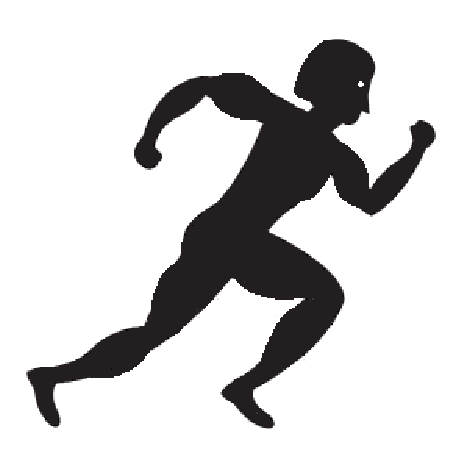
\includegraphics[width=0.3cm]{Hercule}}
\newcommand{\po}{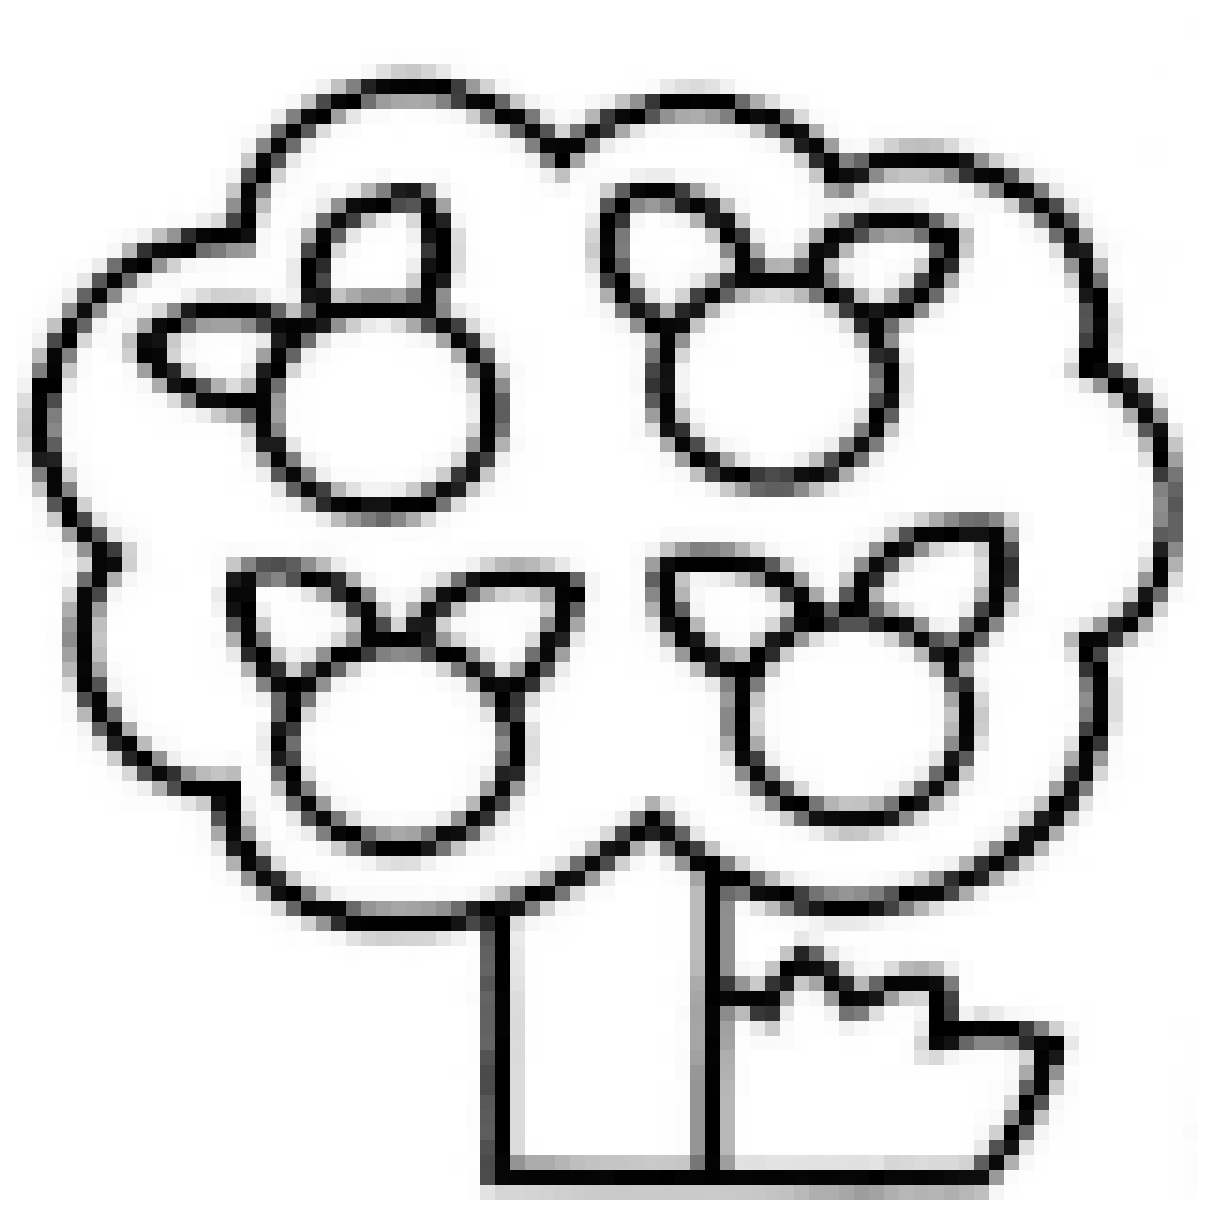
\includegraphics[width=0.3cm]{pommier}}

% Commandes
\newcommand{\dep}{\pspolygon[fillstyle=solid,fillcolor=orange](6,1)(0,1)(0,0)(1,0)(1.25,-0.25)(1.5,0)(6.5,0)(6.5,0.5) \pswedge[fillstyle=solid,fillcolor=orange,linecolor=orange](6,0.5){0.5}{0}{90} \psarc(6,0.5){0.5}{0}{90} \put(0.5,0.3){\footnotesize Démarre}}
\newcommand{\av}[1]{\pspolygon[fillstyle=solid,fillcolor=green](0,0)(1,0)(1.25,-0.25)(1.5,0)(6.5,0)(6.5,1)(1.5,1)(1.25,0.75)(1,1)(0,1) \put(0.5,0.3){\footnotesize Avance de #1}}
\newcommand{\tg}{\pspolygon[fillstyle=solid,fillcolor=yellow](0,0)(1,0)(1.25,-0.25)(1.5,0)(6.5,0)(6.5,1)(1.5,1)(1.25,0.75)(1,1)(0,1) \put(0.5,0.3){\footnotesize Tourne à gauche}}
\newcommand{\td}{\pspolygon[fillstyle=solid,fillcolor=pink](0,0)(1,0)(1.25,-0.25)(1.5,0)(6.5,0)(6.5,1)(1.5,1)(1.25,0.75)(1,1)(0,1) \put(0.5,0.3){\footnotesize Tourne à droite}}
\newcommand{\fin}{\pspolygon[fillstyle=solid,fillcolor=orange](0,0)(6,0)(6.5,0.5)(6.5,1)(1.5,1)(1.25,0.75)(1,1)(0,1)(0,0) \pswedge[fillstyle=solid,fillcolor=orange,linecolor=orange](6,0.5){0.5}{-90}{0} \psarc(6,0.5){0.5}{-90}{0} \put(0.5,0.3){\footnotesize Prends les pommes}}

% Fourmi
\newcommand{\fourmi}[3]{\rput{#3}(#1,#2){\psdot[linecolor=red,dotstyle=triangle*,linewidth=1mm](0,0)}}
\newcommand{\cub}{\psframe[fillstyle=solid,fillcolor=black](0,0)(1,1)}

\chapter{Repérage et\\déplacements}
\label{S05}


%%%%%%%%%%%%%%%%%%%%%%%%%%%%%%%%%%%%%%
\begin{prerequis}
   \begin{itemize}
      \item[\com] (Se) repérer sur une droite graduée, dans le plan muni d'un repère orthogonal.
      \item[\com] Première approche des algorithmes et de la programmation.
   \end{itemize}
\end{prerequis}

\vfill

\begin{debat}[Débat : la fourmi de Langton : que se passe-t-il ensuite ?] 
   La {\bf fourmi de Langton}, du nom de son inventeur scientifique américain {\it Christopher Langton}, est un petit programme informatique inventé vers la fin des années 1980. Il consiste en un automate qui se déplace dans un quadrillage suivant des règles simples. Il modélise le fait qu'un ensemble de comportements élémentaires peut donner lieu à un comportement complexe.
   \begin{center}
      {\psset{unit=0.25}
      \begin{pspicture}(0,0)(13,13)
         \fourmi{6.5}{6.5}{-90}
         \rput(2,0){\cub} \rput(3,0){\cub}
         \rput(1,1){\cub} \rput(2,1){\cub} \rput(9,1){\cub} \rput(10,1){\cub}
         \rput(0,2){\cub} \rput(2,2){\cub} \rput(3,2){\cub} \rput(5,2){\cub} \rput(8,2){\cub} \rput(11,2){\cub}
         \rput(0,3){\cub} \rput(3,3){\cub} \rput(5,3){\cub} \rput(6,3){\cub} \rput(7,3){\cub} \rput(9,3){\cub} \rput(10,3){\cub} \rput(11,3){\cub}
         \rput(1,4){\cub} \rput(3,4){\cub} \rput(10,4){\cub} \rput(12,4){\cub}
         \rput(3,5){\cub} \rput(4,5){\cub} \rput(8,5){\cub} \rput(9,5){\cub}
         \rput(3,6){\cub} \rput(4,6){\cub} \rput(5,6){\cub} \rput(7,6){\cub} \rput(8,6){\cub} \rput(9,6){\cub}
         \rput(3,7){\cub} \rput(4,7){\cub} \rput(8,7){\cub} \rput(9,7){\cub}
         \rput(0,8){\cub} \rput(2,8){\cub} \rput(9,8){\cub} \rput(11,8){\cub}
         \rput(0,9){\cub} \rput(1,9){\cub} \rput(2,9){\cub} \rput(5,9){\cub} \rput(6,9){\cub} \rput(7,9){\cub} \rput(9,9){\cub} \rput(12,9){\cub}
         \rput(1,10){\cub} \rput(4,10){\cub} \rput(7,10){\cub} \rput(9,10){\cub} \rput(10,10){\cub} \rput(12,10){\cub}
         \rput(2,11){\cub} \rput(3,11){\cub} \rput(10,11){\cub} \rput(11,11){\cub}
         \rput(9,12){\cub} \rput(10,12){\cub}
      \end{pspicture}}
   \end{center}
   \bigskip
   \begin{cadre}[B2][F4]
      \begin{center}
         Vidéo : \href{https://www.youtube.com/watch?v=qZRYGxF6D3w}{\bf La fourmi de Langton}, chaîne YouTube {\it Science étonnante}.
      \end{center}
   \end{cadre}
\end{debat}

\vfill

\textcolor{PartieGeometrie}{\sffamily\bfseries Cahier de compétences} : chapitre 3, exercices 17 ; 18 ; 20 ; 22 ; 23.


%%%%%%%%%%%%%%%%%%%%%%%%%%%%%%%%%%%%%
%%%%%%%%%%%%%%%%%%%%%%%%%%%%%%%%%%%%%
\activites

\begin{activite}[La fourmi de Langton]
   {\bf Objectifs :} suivre un algorithme de déplacement ; se repérer dans le plan dans un repérage relatif.
   \begin{QCM}
      La fourmi de Langton est un automate qui se déplace dans un quadrillage suivant les règles suivantes :
      \begin{itemize}
         \item au départ, toutes les cases sont de la même couleur, ici blanches ;
         \item si la fourmi est sur une case blanche, elle tourne de \udeg{90} vers la droite, change la couleur de la case en noir et avance d'une case ;
         \item si la fourmi est sur une case noire, elle tourne de \udeg{90} vers la gauche, change la couleur de la case en blanc et avance d'une case.
      \end{itemize}
      Compléter dans les quadrillages ci-dessous les quinze premières étapes du déplacement de la fourni.
      \begin{center}
      \psset{unit=0.5,subgriddiv=1,gridlabels=0mm,gridcolor=gray}
      \small
      \begin{pspicture}(0,-0.7)(7,7)
         \psgrid(0,0)(7,7)
         \fourmi{3.5}{3.5}{0}
          \rput(3.5,-0.5){étape 0}
      \end{pspicture}
      \quad
      \begin{pspicture}(0,-0.7)(7,7)
         \psframe[fillstyle=solid,fillcolor=darkgray](3,3)(4,4)
         \psgrid(0,0)(7,7)
         \fourmi{4.5}{3.5}{-90}
         \rput(3.5,-0.5){étape 1}
      \end{pspicture}
      \quad
      \begin{pspicture}(0,-0.7)(7,7)  
         \psframe[fillstyle=solid,fillcolor=darkgray](3,3)(5,4)
         \psgrid(0,0)(7,7)
         \fourmi{4.5}{2.5}{180}
         \rput(3.5,-0.5){étape 2}
      \end{pspicture}
      \quad
      \begin{pspicture}(0,-0.7)(7,7)
         \psgrid(0,0)(7,7)
         \rput(3.5,-0.5){étape 3}
      \end{pspicture}
      \bigskip
      \begin{pspicture}(0,-0.7)(7,7)
         \psframe[fillstyle=solid,fillcolor=darkgray](3,2)(5,4)
         \psgrid(0,0)(7,7)
         \fourmi{3.5}{3.5}{0}
         \rput(3.5,-0.5){étape 4}
      \end{pspicture}
      \quad
      \begin{pspicture}(0,-0.7)(7,7)
         \psgrid(0,0)(7,7)
         \rput(3.5,-0.5){étape 5}
      \end{pspicture}
      \quad
      \begin{pspicture}(0,-0.7)(7,7)
         \psgrid(0,0)(7,7)
         \rput(3.5,-0.5){étape 6}
      \end{pspicture}
      \quad
      \begin{pspicture}(0,-0.7)(7,7)
         \psframe[fillstyle=solid,fillcolor=darkgray](2,3)(3,5)
         \pspolygon[fillstyle=solid,fillcolor=darkgray](3,2)(5,2)(5,4)(4,4)(4,3)(3,3)
         \psgrid(0,0)(7,7)
         \fourmi{3.5}{4.5}{-90}
         \rput(3.5,-0.5){étape 7}
      \end{pspicture}
      \bigskip
      \begin{pspicture}(0,-0.7)(7,7)
         \psgrid(0,0)(7,7)
         \rput(3.5,-0.5){étape 8}
      \end{pspicture}
      \quad
      \begin{pspicture}(0,-0.7)(7,7)
         \psgrid(0,0)(7,7)
         \rput(3.5,-0.5){étape 9}
      \end{pspicture}
      \quad
      \begin{pspicture}(0,-0.7)(7,7)
         \psgrid(0,0)(7,7)
         \rput(3.5,-0.5){étape 10}
      \end{pspicture}
      \quad
      \begin{pspicture}(0,-0.7)(7,7)
         \pspolygon[fillstyle=solid,fillcolor=darkgray](2,2)(5,2)(5,4)(4,4)(4,5)(2,5)(2,4)(3,4)(3,3)(2,3)
         \psgrid(0,0)(7,7)
         \rput(3.5,-0.5){étape 11}
         \fourmi{1.5}{2.5}{90}
      \end{pspicture}
      \bigskip
      \begin{pspicture}(0,0)(7,7)
         \psgrid(0,0)(7,7)
         \rput(3.5,-0.5){étape 12}
      \end{pspicture}
      \quad
      \begin{pspicture}(0,0)(7,7)
         \psgrid(0,0)(7,7)
         \rput(3.5,-0.5){étape 13}
      \end{pspicture}
      \quad
      \begin{pspicture}(0,0)(7,7)
         \psgrid(0,0)(7,7)
         \rput(3.5,-0.5){étape 14}
      \end{pspicture}
      \quad
      \begin{pspicture}(0,0)(7,7)
         \psgrid(0,0)(7,7)
         \rput(3.5,-0.5){étape 15}
      \end{pspicture} 
      \end{center}
   \end{QCM}
\end{activite}


%%%%%%%%%%%%%%%%%%%%%%%%%%%%%%%%%%%%%%%%
%%%%%%%%%%%%%%%%%%%%%%%%%%%%%%%%%%%%%%%%%
\cours 

%%%%%%%%%%%%%%%%%%%%%%%%%%%%%%%%%%%%%%%
\section{Repérer un point dans un repère du plan}

\begin{definition}  
   Un \textbf{repère orthogonal} est constitué de deux axes gradués perpendiculaires et sécants en O.
    \begin{itemize}
      \item O est l'\textbf{origine} du repère ;
      \item la droite horizontale est l'\textbf{axe des abscisses} ;
      \item la droite verticale est l'\textbf{axe des ordonnées}.
   \end{itemize} 
\end{definition}

\medskip

\begin{propriete}
   Dans un repère, un point $M$ est repéré par un couple $(x;y)$ appelé coordonnées du point $M$. \\
   $x$ est l'\textbf{abscisse} du point et $y$ est l'\textbf{ordonnée}.
\end{propriete}

\begin{exemple}[0.65]
   \psset{unit=0.65}
   \begin{pspicture}(-5,-3.5)(9,4)
      \psgrid[gridlabels=0,subgriddiv=0,gridcolor=lightgray!70](-4,-3)(4,3)
      \pstGeonode[PosAngle=45](3,1.5){A}(-2,2){B}(-3,-2){C}(2.5,-1.5){D}
      \rput(-0.3,-0.3){\small $O$}
      \rput[l](4.5,0){\textcolor{A1}{axe des abscisses}}
      \rput(0,3.5){\textcolor{B1}{axe des ordonnées}}
      \rput[l](4.5,-2.5){origine du repère}
      \footnotesize
      \psaxes[yAxis=false,linecolor=A1,labels=none]{->}(0,0)(-4,0)(4,0)
      \multido{\n=-4+1}{4}{\rput(\n,-0.4){\textcolor{A1}{\n}}}
      \multido{\n=1+1}{4}{\rput(\n,-0.4){\textcolor{A1}{\n}}}
      \psaxes[xAxis=false,linecolor=B1,labels=none]{->}(0,0)(0,-3)(0,3)
      \multido{\n=-3+1}{3}{\rput(-0.4,\n){\textcolor{B1}{\n}}}
      \multido{\n=1+1}{3}{\rput(-0.4,\n){\textcolor{B1}{\n}}}
      \psline[linestyle=dashed]{->}(4,-2.5)(2,-2.5)(0.1,-0.1)
   \end{pspicture}
   \correction
      Les coordonnées des points \\
      $O, A, B, C$ et $D$ sont : \\
      \begin{itemize}
         \item $O(\textcolor{A1}{0}\,;\textcolor{B1}{0})$
         \item $A(\textcolor{A1}{3}\,;\textcolor{B1}{1,5})$
         \item $B(\textcolor{A1}{-2}\,;\textcolor{B1}{2})$
         \item $C(\textcolor{A1}{-3}\,;\textcolor{B1}{-2})$
         \item $D(\textcolor{A1}{2,5}\,;\textcolor{B1}{-1,5})$
      \end{itemize}
\end{exemple}


%%%%%%%%%%%%%%%%%%%%%%%%%%%%%%%%%%%%%%%
\section{Se déplacer}
 
\begin{methode}[Langages de déplacement]
   Pour se déplacer dans le plan, il existe principalement deux langages de déplacement :
   \begin{itemize}
      \item le langage {\bf absolu} composé de mots de vocabulaire du type : \og haut \fg{}, \og bas \fg{}, \og droite \fg{} et \og gauche \fg. Le déplacement se fait comme si on se plaçait en vue du dessus ;
      \item le langage {\bf relatif} composé de mots de vocabulaire du type : \og avancer \fg{}, \og tourner à droite \fg{} et \og tourner à gauche \fg. C'est ici le point de vue de l'observateur qui est adopté.
   \end{itemize}
   \exercice
   Coder ce déplacement :
   \begin{center}
   \psset{unit=0.7}
   \begin{pspicture}(0,-1)(5,4)
      \psgrid[subgriddiv=1,gridlabels=0mm](0,-1)(5,4)
      \psset{linecolor=A1,arrowsize=3mm,linewidth=0.5mm}
      \psdots(0.5,0.5)(3.5,2.5)     
      \psline{->}(0.5,0.5)(2.5,0.5)(2.5,2.5)(3.5,2.5)
   \end{pspicture}
   \end{center}
   \correction
   \begin{minipage}{4cm}
      Avec le langage absolu : \\
      \og droite \\
      droite \\
      haut \\
      haut \\
      droite \fg \\ [5mm]
   \end{minipage}
   \qquad
   \begin{minipage}{4cm}   
     Avec le langage relatif : \\ [1mm]
     \og avancer \\
     avancer \\
     tourner à gauche \\
     avancer \\
     avancer \\
     tourner à droite \\
     avancer \fg
   \end{minipage}
\end{methode}


%%%%%%%%%%%%%%%%%%%%%%%%%%%%%%%%%%%%
%%%%%%%%%%%%%%%%%%%%%%%%%%%%%%%%%%%%
\exercicesbase

\begin{colonne*exercice}

\serie{Se repérer dans le plan} %%%%%

\begin{exercice} %1
  Lire puis écrire les coordonnées des points A à L.
  {\psset{unit=0.37}
  \begin{center}
  \begin{pspicture}(-9,-10)(9,10)
   \psgrid[gridlabels=0,subgriddiv=0,gridcolor=lightgray](-9,-10)(9,10)
      \psaxes[labels=none,ticks=none]{->}(0,0)(-9,-10)(9,10)
      \psline(2,-0.2)(2,0.2)
      \psline(-0.2,2)(0.2,2)
      \small
      \rput(-0.4,-00.4){$O$}
      \rput(2,-0.5){1}
      \rput(-0.5,2){1}
      \pstGeonode[PointSymbol=+,PosAngle=45,linewidth=1mm](3,3){A}(-4,7){B}(-8,-7){C}(7,-3){D}(6,9){E}(-8,2){F}(-2,-4){G}(2,-6){H}(8,0){I}(0,5){J}(-4;0){K}(0,-8){L}
   \end{pspicture}
   \end{center}}
\end{exercice}

\begin{corrige}
   \begin{colitemize}{3}
      \item \blue $A(1,5\,;\,1,5)$
      \item \blue $B(-2\,;\,3,5)$
      \item \blue $C(-4\,;\,-3,5)$
      \item \blue $D(3,5\,;\,-1,5)$
      \item \blue $E(3\,;\,4,5)$
      \item \blue $F(-4\,;\,1)$
      \item \blue $G(-1\,;\,-2)$
      \item \blue $H(1\,;\,-3)$
      \item \blue $I(4\,;\,0)$
      \item \blue $J(0\,;\,2,5)$
      \item \blue $K(-2\,;\,0)$
      \item \blue $L(0\,;\,-4)$
   \end{colitemize}
   \vspace*{-5mm}
\end{corrige}


\begin{exercice} %2
   On considère les points de coordonnées : \\
   {\hautab{1.2}
   \begin{tabular}{p{1.6cm}p{1.6cm}p{1.6cm}p{1.6cm}}
      $M(-9\,;-5)$ & $N(-4\,;0)$ & $O'(2,5\,;7)$ & $P(5\,;3)$ \\
      $Q(-1\,;-1)$ & $R(2\,;-3)$ & $S(5\,;-2)$ & $T(-6,5\,;-2)$ \\
      $U(-1\,;-4)$ & $V(2\,;0)$ & $W(-6,5\,;4)$ & $X(-9\,,0)$ \\
      $Y(-4\,;-5)$ & $Z(-6,5\,;-1)$ & & \\
   \end{tabular}}
   \begin{enumerate}
      \item Créer un repère orthogonal en prenant un centimètre pour une unité qui puisse contenir tous les points.
      \item Placer les points dans le repère.
      \item Relier dans l'ordre les points suivants :
      \begin{itemize}
         \item $W-X-M-Y-N-W-O'-P-S-Y$.
         \item $U-Q-V-R$.
         \item $X-N-P$.
         \item Tracer le cercle de centre $T$ passant par $Z$.
      \end{itemize}
      Chaineze reconnait un dessin familier. Quel est-il ?
   \end{enumerate}
\end{exercice}

\begin{corrige}
   Chaineze reconnait le dessin d'{\blue une maison}. \\
   {\psset{unit=0.4,PointSymbol=none}
   \begin{pspicture}(-10,-7)(6,8.5)
   \psgrid[gridlabels=0,subgriddiv=0,gridcolor=lightgray](-10,-6)(6,8)
      \psaxes[labels=none,ticks=none]{->}(0,0)(-10,-6)(6,8)
      \psline(1,-0.2)(1,0.2)
      \psline(-0.2,1)(1.2,2)
      \footnotesize
      \rput(-0.4,-00.4){$O$}
      \rput(1,0.5){1}
      \rput(-0.5,1){1}
      \psset{linecolor=blue}
      \pstGeonode[PosAngle={90,135,-135,-45,50},CurveType=polygon](-6.5,4){W}(-9,0){X}(-9,-5){M}(-4,-5){Y}(-4,0){N}
      \pstGeonode[PosAngle=45,CurveType=polyline](2.5,7){O'}(5,3){P}(5,-2){S}
      \pstLineAB{W}{O'}
      \pstLineAB{S}{Y}
      \pstGeonode[PosAngle={-90,135,45,-45},CurveType=polyline](-1,-4){U}(-1,-1){Q}(2,0){V}(2,-3){R}
      \pstLineAB{X}{N}
      \pstLineAB{N}{P}
      \pstGeonode(-6.5,-2){T}(-6.1,-1){Z}
      \psdot(-6.5,-2)
      \pstCircleOA{T}{Z}
   \end{pspicture}}
\end{corrige}

\medskip

\begin{exercice} %3
   On se place dans un repère orthogonal d'origine $O$ et d'unité \ucm{1}.
   \begin{enumerate}
      \item Placer le point $A$ de coordonnées $(3,5\,;1,5)$.
      \item Placer le point $B$ symétrique du point $A$ par rapport à l'axe des abscisses. Quelles sont ses coordonnées ?
      \item Placer le point $C$ symétrique du point $B$ par rapport à l'axe des ordonnées. Quelles sont ses coordonnées ?
      \item Placer le point $D$ symétrique du point $C$ par rapport à l'axe des abscisses. Quelles sont ses coordonnées ?
      \item Quelle est la nature du quadrilatère $ABCD$ ?
   \end{enumerate}
\end{exercice}

\begin{corrige}
   On obtient un {\blue rectangle}. \\
   {\psset{unit=0.8}
   \begin{pspicture}(-4,-2)(4,2.2)
      \footnotesize
      \psgrid[gridlabels=0,subgriddiv=2,gridcolor=lightgray](-4,-2)(4,2)
      \pstGeonode[PointSymbol=none,PosAngle={45,-45,-135,135},CurveType=polygon,linecolor=blue](3.5,1.5){A}(3.5,-1.5){B}(-3.5,-1.5){C}(-3.5,1.5){D}
      \psaxes[labels=none,ticks=none]{->}(0,0)(-4,-2)(4,2)
      \psline(1,-0.2)(1,0.2)
      \psline(-0.2,1)(0.2,1)
      \rput(-0.4,-00.4){$O$}
      \rput(1,0.5){1}
      \rput(-0.5,1){1}
   \end{pspicture}} \\
   {\blue $B(3,5\,;-1.5)\,; C(-3,5\,;-1.5)\,;D(-3,5\,;1.5)$} \\
\end{corrige}


\serie{Algorithmes de déplacement} %%%

\begin{exercice} %4
   Tracer les figures obtenues lorsque l'on exécute les programmes suivants avec scratch. \\
   Pour chaque cas, donner la nature de la figure obtenue. \\
   {\it On représentera l'unité par \umm{1} sur le cahier.}
   \bigskip
   \begin{enumerate}
      \item
      \begin{center}
         \begin{scratch}
            \blockinit{quand \greenflag est cliqué}
            \blockpen{stylo en position d'écriture}
            \blockrepeat{répéter \ovalnum{3} fois}
               {
               \blockmove{avancer de \ovalnum{40}}
               \blockmove{tourner \turnleft{} de \ovalnum{120} degrés}
               }
         \end{scratch}
      \end{center}
      \bigskip
      \item 
      \begin{center}
         \begin{scratch}
            \blockinit{quand \greenflag est cliqué}
            \blockpen{stylo en position d'écriture}
            \blockrepeat{répéter \ovalnum{2} fois}
               {
               \blockmove{avancer de \ovalnum{20}}
               \blockmove{tourner \turnright{} de \ovalnum{90} degrés}
               \blockmove{avancer de \ovalnum{80}}
               \blockmove{tourner \turnright{} de \ovalnum{90} degrés}
               }
         \end{scratch} \\ [3mm]
      \end{center}
      \bigskip
      \item 
      \begin{center}
         \begin{scratch}
            \blockinit{quand \greenflag est cliqué}
            \blockpen{stylo en position d'écriture}
            \blockrepeat{répéter \ovalnum{2} fois}
               {
               \blockmove{avancer de \ovalnum{30}}
               \blockmove{tourner \turnright{} de \ovalnum{50} degrés}
               \blockmove{avancer de \ovalnum{30}}
               \blockmove{tourner \turnright{} de \ovalnum{130} degrés}
               }
         \end{scratch}
      \end{center}
   \end{enumerate}
\end{exercice}

\begin{corrige}
   \ \\ [-3mm]
   {\psset{unit=0.8,linecolor=blue}
   \begin{pspicture}(0,0)(8,8)                                                                              
      \psgrid[gridlabels=0,subgriddiv=0,gridcolor=lightgray](0,0)(8,8)
      \pspolygon(0,4)(4,4)(2,7.46)
      \rput(2,5.25){\textcolor{G1}{\bf 1)} \blue triangle}
      \rput(2,4.75){\blueéquilatéral}
      \psframe(6,0)(8,8)
      \rput(7,4){\textcolor{G1}{\bf 2)} \blue rectangle}
      \pspolygon(0,3)(3,3)(4.93,0.7)(1.93,0.7)
      \rput(2.5,1.8){\textcolor{G1}{\bf 3)} \blue losange}
   \end{pspicture}}
\end{corrige}

\pagebreak

\begin{exercice} %5
   L'image suivante représente la position obtenue au déclenchement du bloc \og Départ \fg{} d'un programme. \\
   L'arrière-plan est constitué de points espacés de 40 unités. Le chat a pour coordonnées $(-120\,;\,-80)$. \\
   Le but du jeu est de positionner le chat sur la balle représentée par le petit disque.
   \begin{center}
   {\psset{unit=0.4}
   \begin{pspicture}(-6,-3.3)(6,4.3)
      \multido{\n=-6+1}{13}{
      \multido{\na=-4+1}{9}{\psdots[dotscale=0.5](\n,\na)}}
      \psaxes[Dx=10,Dy=10]{->}(0,0)(-6,-4)(6,4)
      \uput[dl](0,0){O}
      \psdots[dotscale=2](4,3)
      \rput(-3,-2){Chat}
   \end{pspicture}}
   \end{center}
   \begin{enumerate}
      \item Quelles sont les coordonnées du centre de la balle représentée dans cette position?
      \item Dans cette question, le chat est dans la position obtenue au déclenchement du bloc départ. \\
      Voici le script du lutin \og chat \fg{} qui se déplace. \\ [3mm]
      \hspace*{-9mm}
      {\small
      \begin{scratch}
         \blockinit{Quand \greenflag est cliqué}
         \blockmove{Départ}
      \end{scratch}
      \begin{scratch}
         \blockinit{Quand \selectmenu{n'importe quoi}  est cliqué}{
            \blockifelse{si \selectmenu{Balle} touchée alors}{
               \blocklook{dire \txtbox{Je t'ai attrapée} pendant \ovalnum{2} secondes}
               \blockmove{Départ}}
               {}}
      \end{scratch}
      \smallskip
      
      \hspace*{-9mm}
      \begin{scratch}
         \blockinit{Quand flèche gauche  est cliqué}
         \blockvariable{ajouter \ovalnum{-40} à \selectmenu{x}}
      \end{scratch} 
      \quad
      \begin{scratch}
         \blockinit{Quand flèche droite  est cliqué}
         \blockvariable{ajouter \ovalnum{80} à \selectmenu{x}}
      \end{scratch}   
      \smallskip
      
      \hspace*{-9mm}
      \begin{scratch}
         \blockinit{Quand flèche haut  est cliqué}
         \blockvariable{ajouter \ovalnum{80} à \selectmenu{y}}
      \end{scratch}
      \qquad
      \begin{scratch}
         \blockinit{Quand flèche bas  est cliqué}
         \blockvariable{ajouter \ovalnum{-40} à \selectmenu{y}}
      \end{scratch}
      }
      \medskip
      \begin{enumerate}
         \item Expliquer pourquoi le chat ne revient pas à sa position de départ si le joueur appuie sur la touche $\to$ puis sur la touche $\gets$.
         \item Le joueur appuie sur la succession de touches suivante : $\to$ $\to$  $\uparrow$ $\gets$ $\downarrow$. Quelles sont les coordonnées $x$ et $y$ du chat après ce déplacement ? Justifier.
         \item Parmi les propositions ci-dessous, laquelle permet au chat d'atteindre la balle ? \medskip
      \end{enumerate}
      \hspace*{-5mm}
      {\small
      \hautab{1.2}
      \begin{tabular}{|c|c|c|}
         \hline
         déplacement 1 & déplacement 2 & déplacement 3\\ \hline
         $\to \to \to \to \to \to \to \uparrow\uparrow\uparrow\uparrow\uparrow$
         &
         $\to\to\to \uparrow\uparrow\uparrow \to \downarrow \gets$
         &
         $\uparrow \to \uparrow \to \uparrow \to \to \downarrow \downarrow$ \\
         \hline
      \end{tabular}}
      \smallskip
      \item Que se passe-t-il quand le chat atteint la balle ?
   \end{enumerate}
\end{exercice}

\begin{corrige}
   \ \\ [-5mm]
   \begin{enumerate}
      \item La balle est située à quatre espaces vers la droite, soit $4\times40$ unités = 160 unités et trois espaces vers le haut, soit $3\times40$ unités = 120 unités. \\
      Ses coordonnées sont donc {\blue (160\,;\,120)}.
      \item \\
      \begin{enumerate}
         \item La touche $\to$ ajoute 80 à l'abscisse $x$ ; la touche $\gets$ ajoute $-40$ à l'abscisse $x$ ; donc, la succession $\to \, \gets$ ajoute $80+(-40) =40$ à l'abscisse $x$. \\
         Le chat a finalement \og avancé \fg{} de 40 unités vers la droite, donc {\blue il ne revient pas à sa position de départ}. 
         \item On résume dans un tableau les différents déplacements : \\ \smallskip
            {\hautab{1.5}
            \begin{tabular}{|*{7}{c|}}
               \hline
               & départ & $\to$ & $\to$ & $\uparrow$ & $\gets$ & $\downarrow$ \\
               \hline
               $x$ & $-120$ & $-40$ & 40 & 40 & 0 & 0 \\
               \hline 
               $y$ & $-80$ & $-80$ & $-80$ & 0 & 0 & $-40$ \\
               \hline
            \end{tabular}} \\ \smallskip
         Les coordonnées du chat après ces cinq déplacements sont {\blue $(0\,;\,-40)$}.
         \item Seul le {\blue déplacement 2} permet au chat d'attraper la balle.
      \end{enumerate}
      \setcounter{enumi}{2}
      \item Lorsque le chat atteint la balle, {\blue il dit \og Je t'ai attrapée \fg{} pendant 2 secondes}, puis il retourne au départ. 
   \end{enumerate}
\end{corrige}


\begin{exercice} %6
   Un programme permet à un robot de se déplacer sur les cases d'un quadrillage. Chaque case atteinte est colorée en gris. \\
Au début d'un programme, toutes les cases sont blanches, le robot se positionne sur une case de départ indiquée par un \og {\bf d} \fg{} et la colore aussitôt en gris. \\
Le robot se déplace suivant un programme grâce à un langage absolu dont le vocabulaire est
   \begin{center}
      \og S (south) ; E (east) ; N (north) ; W (west) \fg.
   \end{center}
   Voici des exemples de programmes et leurs effets :
   \begin{center}
   \begin{tabular}{|p{1.5cm}|C{2.5}|C{2.7}|}
      \hline
      1W
      &
      Le robot avance de 1 case vers l'ouest.
      &
      {\psset{unit=0.5cm}
      \begin{pspicture}(1,2)(3,3.5)
         \psframe[fillstyle=solid,fillcolor=lightgray](1,1)(3,2)
         \psgrid[gridlabels=0,subgriddiv=1,gridcolor=gray](0,0)(4,3)
         \rput(2.5,1.5){\textbf{d}}
      \end{pspicture}} \\
      \hline
      2E 1W 2N
      &
      Le robot avance de 2 cases vers l'est, puis de 1 case vers l'ouest,
puis de 2 cases vers le nord.
      &
      {\psset{unit=0.5cm}
      \begin{pspicture}(0,4.4)(5,6)
         \pspolygon[fillstyle=solid,fillcolor=lightgray](1,1)(4,1)(4,2)(3,2)(3,4)(2,4)(2,2)(1,2)
         \psgrid[gridlabels=0,subgriddiv=1,gridcolor=gray](5,5)
         \rput(1.5,1.5){\textbf{d}}
      \end{pspicture}} \\
      \hline
   \end{tabular}
   \end{center}
   \begin{enumerate}
      \item Voici un programme :
      \begin{center}
         1W 2N 2E 4S 2W
      \end{center}
      On souhaite dessiner le motif obtenu avec ce programme. Sur votre copie, réaliser ce motif en utilisant des carreaux, comme dans les exemples précédents. On marquera un \og \textbf{d} \fg{} sur la case de départ.
      \item On fait fonctionner un programme qui dessine le motif suivant :
      \begin{center}
      {\psset{unit=0.6cm}
      \begin{pspicture}(-0.5,-0.2)(8,3.7)
         \pspolygon[fillstyle=solid,fillcolor=lightgray](0,2)(1,2)(1,1)(2,1)(2,2)(3,2)(3,1)(4,1)(4,2)(5,2)(5,1)(6,1)(6,2)(7,2)(7,0)(0,0)
         \psgrid[gridlabels=0,subgriddiv=1,gridcolor=gray](-1,-1)(8,3)
         \rput(0.5,1.5){\textbf{d}}
      \end{pspicture}}
      \end{center}
      \begin{enumerate}
         \item Proposer un programme permettant de dessiner ce motif.
         \item Comment pourrait-on faire évoluer l'écriture de ce programme afin qu'il soit plus compact ?
      \end{enumerate}
   \end{enumerate}
   \hfill{\footnotesize\it Source : exercices inspirés d'épreuves du DNB}
   \end{exercice}

\begin{corrige}
   \ \\ [-5mm]\begin{enumerate}
      \item On obtient le {\blue dessin d'un 9} : \\
         {\psset{unit=0.5cm,linecolor=white,fillstyle=solid,fillcolor=white}
         \begin{pspicture}(-4,1)(4,7.5)
            \psframe[fillcolor=lightgray](1,1)(4,6)
            \psframe(1,2)(3,3)          
            \psframe(2,4)(3,5)
            \psgrid[gridlabels=0,subgriddiv=1,gridcolor=gray](5,7)
            \rput(1.5,1.5){\textbf{d}}
         \end{pspicture}}
      \item \\
      \begin{enumerate}
         \item Le motif peut être programmé grâce à la suite : \\
            {\blue 1S 2E 1N 1S 2E 1N 1S 2E 1N}
         \item On peut introduire une boucle de répétition, par exemple : {\blue 3$\times$(1S 2E 1N)}
      \end{enumerate}
   \end{enumerate}

\bigskip 
\corec{Le jeu des dominogrammes}
\medskip

Les dominos s'enchaînent dans l'ordre de gauche à droite et de haut en bas soit : \\
\ding{40} -- \ding{110} -- \ding{57} -- \ding{52} -- \ding{70} -- \ding{74} -- \ding{87} -- \ding{115}
\end{corrige}

\end{colonne*exercice}


%%%%%%%%%%%%%%%%%%%%%%%%%%%%%%%%%
%%%%%%%%%%%%%%%%%%%%%%%%%%%%%%%%%
\Recreation

\enigme[Le jeu des dominogrammes]
   
   {\bf But du jeu} : en groupe, faire une chaîne fermée avec les huit cartes de domino. \\
   {\bf Règle du jeu} : chaque domino est basé sur {\it Les douze travaux d'Hercule}, et notamment le travail n\degre11 dans lequel Hercule doit dérober les pommes d'or du jardin d'Hespérides. Le côté gauche comporte un quadrillage avec des cases noirs que l'on ne peut pas traverser, le personnage d'Hercule (orienté) et le pommier du jardin d'Hespérides. Le côté droit comporte un programme de déplacement d'Hercule. L'objectif est d'associer un programme d'un domino avec un quadrillage d'un autre domino. Les huit dominos doivent créer une chaine fermée. \\
   {\psset{unit=0.4}
   \begin{pspicture}(-1,-1)(19,10) % jaune 1
      \psframe(-1,-1)(19,9)
      \psline(9,-1)(9,9)
      \psgrid[subgriddiv=1,gridlabels=0](0,0)(8,8)
      \put(3.1,4.1){\ho} \put(7.1,6.1){\po}
      \put(1,1){\cn} \put(2,3){\cn} \put(3,2){\cn} \put(2,4){\cn}  \put(5,5){\cn} \put(7,2){\cn} \put(5,7){\cn} \put(6,0){\cn} \put(1,6){\cn}     
      \put(10,7){\dep}
      \put(10,6){\av{3}}
      \put(10,5){\td}
      \put(10,4){\av{1}}
      \put(10,3){\tg}
      \put(10,2){\av{1}}
      \put(10,1){\fin}
      \put(18,8){\ding{40}}
   \end{pspicture}
   \;
   \begin{pspicture}(-1,-1)(19,10) % jaune 2
      \psframe(-1,-1)(19,9)
      \psline(9,-1)(9,9)
      \psgrid[subgriddiv=1,gridlabels=0](0,0)(8,8)
      \rput{90}(3.5,2.5){\ho} \put(4.1,6.1){\po}
      \put(1,2){\cn} \put(4,3){\cn} \put(3,0){\cn} \put(2,7){\cn}  \put(5,6){\cn} \put(1,2){\cn} \put(0,7){\cn} \put(6,2){\cn} \put(1,3){\cn}     
      \put(10,7){\dep}
      \put(10,6){\td}
      \put(10,5){\av{4}}
      \put(10,4){\tg}
      \put(10,3){\av{3}}
      \put(10,2){\tg}
      \put(10,1){\av{1}}
      \put(10,0){\fin}
      \put(18,8){\ding{110}}
   \end{pspicture}

   \medskip
   \begin{pspicture}(-1,-1)(19,9) % jaune 3
      \psframe(-1,-1)(19,9)
      \psline(9,-1)(9,9)
      \psgrid[subgriddiv=1,gridlabels=0](0,0)(8,8)
      \put(5.1,3.1){\reflectbox{\ho}} \put(2.1,6.1){\po}
      \put(6,6){\cn} \put(3,3){\cn} \put(3,6){\cn} \put(2,5){\cn}  \put(3,5){\cn} \put(4,2){\cn} \put(1,3){\cn} \put(0,0){\cn} \put(2,5){\cn}     
      \put(10,7){\dep}
      \put(10,6){\av{7}}
      \put(10,5){\tg}
      \put(10,4){\av{7}}
      \put(10,3){\tg}
      \put(10,2){\av{7}}
      \put(10,1){\fin}
      \put(18,8){\ding{57}}
   \end{pspicture}
   \;
   \begin{pspicture}(-1,-1)(19,9) % jaune 4
      \psframe(-1,-1)(19,9)
      \psline(9,-1)(9,9)
      \psgrid[subgriddiv=1,gridlabels=0](0,0)(8,8)
      \put(0.1,0.1){\ho} \put(0.1,7.1){\po}
      \put(5,3){\cn} \put(4,3){\cn} \put(3,6){\cn} \put(0,6){\cn}  \put(5,5){\cn} \put(2,1){\cn} \put(2,5){\cn} \put(6,2){\cn} \put(1,3){\cn}     
      \put(10,7){\dep}
      \put(10,6){\av{3}}
      \put(10,5){\tg}
      \put(10,4){\td}
      \put(10,3){\av{2}}
      \put(10,2){\tg}
      \put(10,1){\av{2}}
      \put(10,0){\fin}
      \put(18,8){\ding{52}}
   \end{pspicture}

   \medskip
   \begin{pspicture}(-1,-1)(19,9) % jaune 5
      \psframe(-1,-1)(19,9)
      \psline(9,-1)(9,9)
      \psgrid[subgriddiv=1,gridlabels=0](0,0)(8,8)
      \rput{90}(5.5,0.5){\ho} \put(3.1,5.1){\po}
      \put(1,1){\cn} \put(0,3){\cn} \put(4,2){\cn} \put(3,4){\cn}  \put(5,6){\cn} \put(7,3){\cn} \put(5,7){\cn} \put(6,1){\cn} \put(1,7){\cn}     
      \put(10,7){\dep}
      \put(10,6){\av{6}}
      \put(10,5){\td}
      \put(10,4){\av{3}}
      \put(10,3){\td}
      \put(10,2){\av{2}}
      \put(10,1){\tg}
      \put(10,0){\fin}
      \put(18,8){\ding{70}}
   \end{pspicture}
   \;
   \begin{pspicture}(-1,-1)(19,9) % jaune 6
      \psframe(-1,-1)(19,9)
      \psline(9,-1)(9,9)
      \psgrid[subgriddiv=1,gridlabels=0](0,0)(8,8)
      \rput{-90}(4.5,7.5){\ho} \put(1.1,3.1){\po}
      \put(0,2){\cn} \put(6,5){\cn} \put(1,0){\cn} \put(2,0){\cn}  \put(3,6){\cn} \put(1,6){\cn} \put(6,7){\cn} \put(6,2){\cn} \put(1,7){\cn}     
      \put(10,7){\dep}
      \put(10,6){\av{2}}
      \put(10,5){\tg}
      \put(10,4){\av{1}}
      \put(10,3){\fin}
      \put(18,8){\ding{74}}
   \end{pspicture}

   \medskip
   \begin{pspicture}(-1,-1)(19,9) % jaune 7
      \psframe(-1,-1)(19,9)
      \psline(9,-1)(9,9)
      \psgrid[subgriddiv=1,gridlabels=0](0,0)(8,8)
      \put(7.1,7.1){\reflectbox{\ho}} \put(5.1,6.1){\po}
      \put(6,6){\cn} \put(2,3){\cn} \put(0,6){\cn} \put(4,2){\cn}  \put(3,7){\cn} \put(1,2){\cn} \put(0,3){\cn} \put(7,2){\cn} \put(2,5){\cn}
      \put(10,7){\dep}
      \put(10,6){\av{2}}
      \put(10,5){\tg}
      \put(10,4){\tg}
      \put(10,3){\tg}
      \put(10,2){\tg}
      \put(10,1){\av{2}}
      \put(10,0){\fin}
      \put(18,8){\ding{87}}
   \end{pspicture}
   \;
   \begin{pspicture}(-1,-1)(19,9) % jaune 8
      \psframe(-1,-1)(19,9)
      \psline(9,-1)(9,9)
      \psgrid[subgriddiv=1,gridlabels=0](0,0)(8,8)
      \rput{90}(2.5,3.5){\ho} \put(2.1,7.1){\po}
      \put(5,3){\cn} \put(3,3){\cn} \put(3,6){\cn} \put(0,5){\cn}  \put(7,5){\cn} \put(2,1){\cn} \put(2,0){\cn} \put(6,2){\cn} \put(1,3){\cn}     
   \put(10,7){\dep}
      \put(10,6){\av{1}}
      \put(10,5){\tg}
      \put(10,4){\av{2}}
      \put(10,3){\td}
      \put(10,2){\av{2}}
      \put(10,1){\av{1}}
      \put(10,0){\fin}
      \put(18,8){\ding{115}}
   \end{pspicture}}
   \bigskip
   
   Lorsque le groupe a réussi la mission, passer au niveau supérieur avec une autre série de dominos comportant des boucles de répétition.
